\documentclass {article}
\usepackage{graphicx}

\usepackage{algorithm}
\usepackage{algpseudocode}

\begin{document}
\title{Big Graph Tools}
\author{Tian Yong}
\maketitle
\section{Introduction}
There are several choices to implement an algorithm to process a large graph:
\begin{itemize}
  \item Crafting a custom distributed infrastructure. This choice leaves machine learning experts repeatedly design a system and implement it.
  \item Relying on an existing distributed computing platform like MapReduce, which is not suit for graph processing.
  \item Using a single-computer graph algorithm library limiting the scale of problems that can addressed.
  \item Using an parallel graph system, fault tolerance or not.
\end{itemize}
\section{Pregel}
The input to a Pregel computation is a directed graph in
which each vertex is uniquely identified by a string vertex
identifier. Each vertex is associated with a modifiable, user
defined value. The directed edges are associated with their
source vertices, and each edge consists of a modifiable, user
defined value and a target vertex identifier.


Pregel computations consist of a sequence of iterations, called \emph{supersteps}. During a superstep the framework invokes a userdefined function for each vertex, conceptually in parallel.
The function specifies behavior at a single vertex $V$ and a
single superstep $S$. It can read messages sent to $V$ in superstep $S-1$, send messages to other vertices that will be received at superstep $S + 1$, and modify the state of $V$ and
its outgoing edges. Messages are typically sent along outgoing edges, but a message may be sent to any vertex whose
identifier is known.  All communication is from superstep $S$ to superstep $S + 1$. In supersteps, vertex can even change the topology of the graph.

Algorithm termination is based on every vertex voting to
halt. In superstep 0, every vertex is in the active state; all
active vertices participate in the computation of any given
superstep. A vertex deactivates itself by voting to halt. This
means that the vertex has no further work to do unless triggered externally, and the Pregel framework will not execute
that vertex in subsequent supersteps unless it receives a message. If reactivated by a message, a vertex must explicitly deactivate itself again. The algorithm as a whole terminates
when all vertices are simultaneously inactive and there are
no messages in transit. This state transition model is illustrated in figure \ref{SMachine}.


\begin{figure}
  \centering
  % Requires \usepackage{graphicx}
  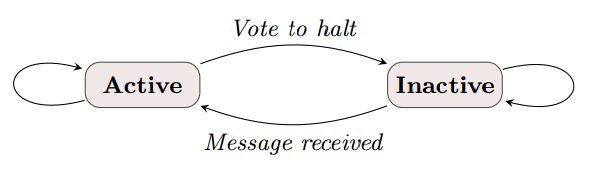
\includegraphics[width=\textwidth]{pregel_vertext_machine.PNG}\\
  \caption{Pregel Vertext State Machine}\label{SMachine}
\end{figure}

Figure \ref{pregel_max} illustrates these concepts using a simple example:
given a strongly connected graph where each vertex contains
a value, it propagates the largest value to every vertex. In
each superstep, any vertex that has learned a larger value
from its messages sends it to all its neighbors. When no
further vertices change in a superstep, the algorithm terminates
\begin{figure}
  \centering
  % Requires \usepackage{graphicx}
  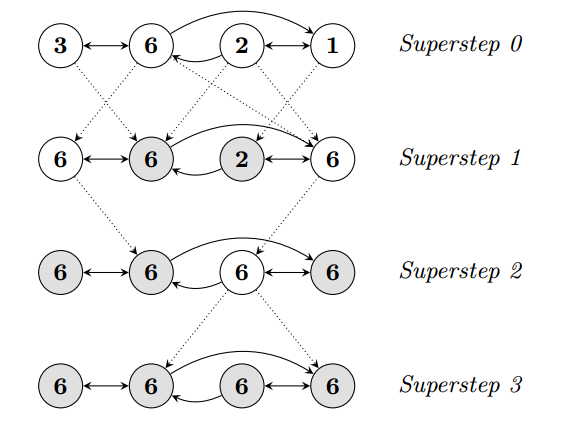
\includegraphics[width=\textwidth]{pregel_max_example.PNG}\\
  \caption{Maximum Value Example. Dotted lines
are messages. Shaded vertices have voted to halt.}\label{pregel_max}
\end{figure}


\subsection{Topology Mutations}
Some graph algorithms need to change the graph's topology. A clustering algorithm, for example, might replace each
cluster with a single vertex, and a minimum spanning tree
algorithm might remove all but the tree edges. User defined function can not only send messages, but also can
issue requests to add or remove vertices or edges.


Multiple vertices may issue conflicting requests in the same
superstep. To solve this problem, Pregel use two mechanisms to achieve
determinism:
\begin{itemize}
  \item Partial ordering. As with messages, mutations become elective in the superstep after the requests were
  issued. Within that superstep removals are performed first, with edge removal before vertex removal. Then additions follow, with vertex addition before edge addition. This partial ordering yields deterministic results for most conflicts.
  \item Handlers. The remaining conflicts are resolved by user-defined handlers. For these conflicts, system have a default random resolution. Butt users with special needs may specify a better conflict resolution policy by defining an appropriate handler method.
\end{itemize}

\section{GraphLab}
GraphLab is a parallel framework for ML which exploits the sparse structure and common computational patterns of ML algorithms. GraphLab
enables ML experts to easily design and implement efficient scalable parallel algorithms by composing problem
specific computation, data-dependencies, and scheduling. GraphLab is implemented with an efficient shared-memory mechanism for it is both ubiquitous and has
few effective high-level abstractions.

\subsection{Data Model}
The GraphLab data model consists of two parts: a directed \emph{data graph} and a \emph{shared data table}. The data graph is arbitrary data block associated
with vertex or edges in a graph while a shared data table(SDT) is an associative map between keys and arbitrary blocks of data to support globally shared state or data.
\subsection{User Defined Computation}
There are two kinds of computation in GraphLab: update and sync. Update functions are permitted to access and modify overlapping contexts in the graph and do local computations. Sync is used to global aggregation and it runs concurrently with update functions.


A GraphLab update function is a stateless user-defined
function which operates on the data associated with small
neighborhoods in the graph and represents the core element
of computation. Given arbitrary vertex $v$, $S_v$ represents the
neighborhood of $v$ which consists of $v$, its adjacent edges
(both inbound and outbound) and its neighboring vertices. And $D_{S_v}$ stands for the data corresponding to the neighborhood $S_v$
. In addition to $D_{S_v}$, update functions also have read-only access, to the shared
data table $T$. An update function $f$ to the vertex $v$ is:
\begin{equation}
  D_{S_v} \leftarrow f(D_{S_v}, T).
\end{equation}

A GraphLab program may consist of
multiple update functions and it is up to the scheduling
model to determine which update functions
are applied to which vertices and in which parallel order.


The sync mechanism aggregates data across all vertices in
the graph and its result is associated with a particular entry int the SDT. To invoke a sync mechanism, user
should provide a key $k$, a \textbf{fold function}(Eq. (\ref{fold_function})), an \textbf{appply function}(Eq. (\ref{apply_function})) as well as an initial value $r^{(0)}_k$ to the SDT.
\begin{equation}\label{fold_function}
r^{i+1}_k \leftarrow Fold_k (D_v, r^{i}_k)
\end{equation}
\begin{equation}\label{apply_function}
  T[k] \leftarrow Apply_k(r_k^{(|V|)})
\end{equation}

When the sync mechanism is invoked, the algorithm in
Alg.\ref{sync_algo} uses the $Fold_k $
function to sequentially aggregate
data across all vertices. The sync mechanism can be set to run periodically in the
background while the GraphLab engine is actively applying update functions or on demand triggered by update
functions or user code. If the sync mechanism is executed
in the background, the resulting aggregated value may not
be globally consistent. Nonetheless, many ML applications
are robust to approximate global statistics.


\begin{algorithm}
\caption{Sync algorithm on k}
\label{sync_algo}
\begin{algorithmic}[1]
\Procedure {SYNC}{$k$, $r_k^{(0)}$}
    \State $t \leftarrow r_k^{(0)}$
    \ForAll {$v \in V$}
        \State $t \leftarrow Fold_k(D_v, t)$
    \EndFor
    \State $T[k] \leftarrow Apply_k(t)$

\EndProcedure


\end{algorithmic}
\end{algorithm}

\subsection{Data Consistency}
Since scopes may overlap, the simultaneous execution of
two update functions can lead to race-conditions resulting
in data inconsistency and even corruption. GraphLab provides
 a choice of three data consistency models which enable the user
  to balance performance and data consistency. The 3 models is illustrated in Figure \ref{graphlab_scope}
   by drawing their exclusion sets as a ring where no two update functions
    may be executed simultaneously if their exclusions sets overlap
\begin{figure}
  \centering
  % Requires \usepackage{graphicx}
  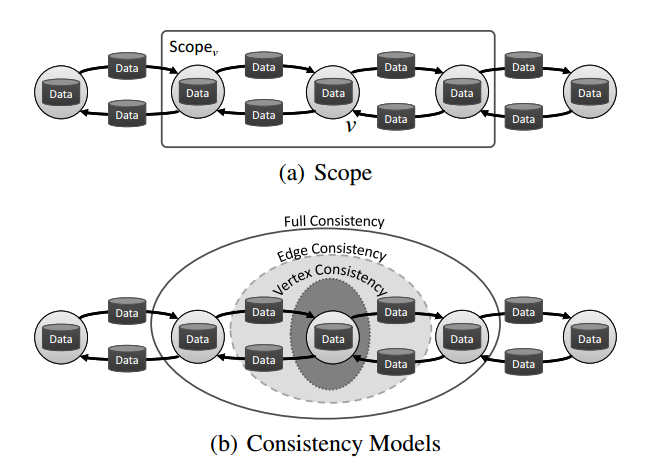
\includegraphics[width=\textwidth]{graphlab_scope}\\
  \caption{(a) The scope, $S_v$ of vertex $v$. (b). Three data consistency
   models.}\label{graphlab_scope}
\end{figure}



\subsection{Scheduling}
The GraphLab update schedule describes the order in
which update functions are applied to vertices and is represented by a parallel data-structure called the scheduler.
The scheduler abstractly represents a dynamic list of tasks
(vertex-function pairs) which are to be executed by the
GraphLab engine. GraphLab framework provides a collection of base schedules to achieve different goals.

GraphLab also provide 2 termination assessment methods. The first method relies on
the scheduler which signals termination when there are no
remaining tasks. The second termination
method relies on user provided termination functions which
examine the SDT and signal when the algorithm has converged.


\section{PowerGraph}
\subsection{Challenges of Natural Graphs}
The sparsity structure of natural graphs presents a unique
challenge to efficient distributed graph-parallel computation. 
One of the hallmark properties of natural graphs is their skewed 
power-law degree distribution: most vertices have relatively few 
neighbors while a few have many neighbors. Under a power-law degree 
distribution the probability that a vertex has degree $d$ is given 
by:
\begin{equation}\label{prob_degree}
  P(d) \propto d^{-\alpha}
\end{equation}
where the exponent $\alpha$ is a positive constant that controls
the ``skewness'' of the degree distribution.


The skewed degree distribution implies that a small
fraction of the vertices are adjacent to a large fraction
of the edges. For example, one percent of the vertices
in the Twitter web-graph are adjacent to nearly half of
the edges. This concentration of edges results in a star-like motif 
which presents challenges, such as work balance, communication and 
storage, for existing graph-parallel abstractions, which factor 
computation over vertices.


\begin{algorithm}
\caption{Vertex-Program Execution Semantics}
\label{vertex_algo}
\begin{algorithmic}[1]
\State \textbf{Input}: Center vertex $u$
\If cached accumulator $a_u$ is empty
    \For neighbor $v$ in gather \_nbrs(u)
    \State $a_u \leftarrow sum(a_u, gather(D_u, D_{(u, v)}, D_v))$
    \EndFor
\EndIf
\State $D_u \leftarrow apply(D_u, a_u)$
\For neighbor v scatter\_nbrs(u)
    \State $(D_{(u, v)}, \Delta a) \leftarrow scatter(D_u, D_{(u,v)}, D_v)$
    \If $a_v$ and $\Delta a$ are not Empty
        \State $a_v \leftarrow sum(a_v, \Delta a)$
    \Else
        \State $a_v \leftarrow$ Empty
    \EndIf
\EndFor
\end{algorithmic}
\end{algorithm}

\subsection{GAS Vertex-Programs}
To address the challenge of computation on power-law graphs, 
PowerGraph abstraction exploits the structure of vertex-programs
and explicitly factors computation over edges instead of vertices.
As a consequence, PowerGraph exposes substantially greater parallelism,
reduces network communication and storage costs, and provides a new
highly effective approach to distributed graph placement.

\begin{figure}
  \centering
  % Requires \usepackage{graphicx}
  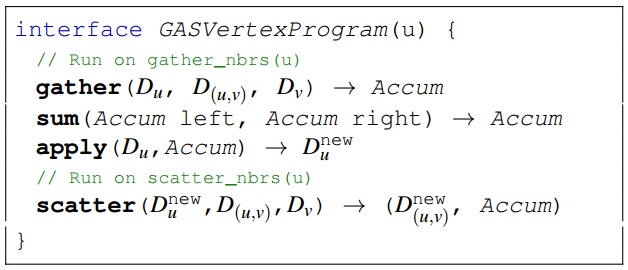
\includegraphics[width=\textwidth]{GAS.png}\\
  \caption{All PowerGraph programs must implement the stateless 
  gather, sum, apply, and scatter functions.}\label{GAS_inter}
\end{figure}


Computation in the PowerGraph abstraction is encoded
as a state-less vertex-program which implements the
GASVertexProgram interface (Fig. \ref{GAS_inter}) and therefore
explicitly factors into the gather, sum, apply, and scatter functions. 
Each function is invoked in stages by the PowerGraph engine following 
the semantics in Alg.\ref{vertex_algo}. By factoring the vertex-program,
the PowerGraph execution engine can distribute a single vertex-program over
multiple machines and move computation to the data.


During the gather phase the gather and sum functions are used as a map and
reduce to collect information about the neighborhood of the vertex.
The gather function is invoked in parallel on the edges adjacent to $u$. The
particular set of edges is determined by $gather\_nbrs$ which can be $none$, 
$in$, $out$, or $all$. The gather function is passed the data on the adjacent
vertex and edge and returns a temporary accumulator (a user defined type).
The result is combined using the commutative and associative sum operation.
The final result $a_u$ of the gather phase is passed to the $apply$ phase and
cached by PowerGraph.


After the $gather$ phase has completed, the $apply$ function takes the final
accumulator and computes a new vertex value $D_u$ which is atomically written
back to the graph. The size of the accumulator $a_u$ and complexity of the 
apply function play a central role in determining the network and storage 
efficiency of the PowerGraph abstraction and should be sub-linear and ideally
constant in the degree.


During the $scatter$ phase, the scatter function is invoked in parallel on 
the edges adjacent to $u$ producing new edge values $D_{(u,v)}$ which are 
written back to the data graph. As with the gather phase, the $scatter\_nbrs$
determines the particular set of edges on which scatter is invoked. The scatter
function returns an optional value $\Delta a$ which is used to dynamically
update the cached accumulator $a_v$ for the adjacent vertex.

\subsection{Delta Chaching}
In many cases a vertex-program will be triggered in response to a change in a
few of its neighbors. The gather operation is then repeatedly invoked on all 
neighbors, many of which remain unchanged, thereby wasting computation cycles.
For many algorithms it is possible to dynamically maintain the result of the 
gather phase $a_u$ and skip the gather on subsequent iterations. The PowerGraph
engine maintains a cache of the accumulator $a_u$ from the previous gather phase
for each vertex. The scatter function can optionally return an additional $\Delta
a$ which is atomically added to the cached accumulator $a_v$ of the neighboring 
vertex $v$ using the sum function. If $\Delta a$ is not returned, then the 
neighbor`s cached $a_v$ is cleared forcing a complete gather on the subsequent
execution of the vertex-program on the vertex $v$. When executing the vertex-program 
on $v$ the PowerGraph engine uses the cached $a_v$ if available, bypassing the 
gather phase.


\subsection{Initiating Future Computation}
The PowerGraph engine maintains a set of active vertices
on which to eventually execute the vertex-program. The
user initiates computation by calling $Activate(v)$ or
$Activateall()$. The PowerGraph engine then proceeds to
execute the vertex-program on the active vertices until
none remain. Once a vertex-program completes the scatter
phase it becomes inactive until it is reactivated.

Vertices can activate themselves and neighboring vertices.
Each function in a vertex-program can only activate vertices
visible in the arguments to that function. 

The order in which activated vertices are executed is up
to the PowerGraph execution engine. The only guarantee
is that all activated vertices are eventually executed. This
flexibility in scheduling enables PowerGraph programs
to be executed both synchronously and asynchronously,
leading to different tradeoffs in algorithm performance,
system performance, and determinism.


\subsection{Distributed Graph Placement}

\begin{figure}
  \centering
  % Requires \usepackage{graphicx}
  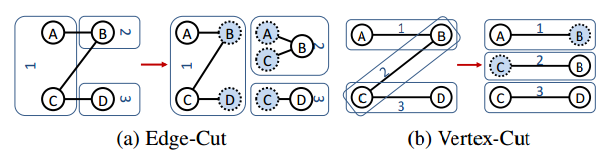
\includegraphics[width=\textwidth]{cut.png}\\
  \caption{(a)An edge-cut and(b)vertex-cut of a graph
  into   three parts. Shaded vertices are ghosts and
  mirrors respectively.}\label{cut}
\end{figure}

The placement of the data-graph structure and data plays
a central role in minimizing communication and ensuring
work balance. A common approach to placing a graph on a
cluster of $p$ machines is to construct a balanced $p$-way
edge-cut (e.g., Fig. \ref{cut}a) in which vertices are evenly
assigned to machines and the number of edges spanning machines
is minimized. Unfortunately, the tools for constructing balanced 
edge-cuts perform poorly on power-law graphs. When the graph
is difficult to partition, both GraphLab and Pregel resort
to hashed (random) vertex placement. While fast and easy to
implement, hashed vertex placement cuts most of the edges. If 
vertices are randomly assigned to $p$ machines then the expected
fraction of edges cut is:
\begin{equation}
  \textbf{E}[\frac{|Edges Cut|}{|E|} = 1 - \frac{1}{p}.
\end{equation}

For a power-law graph with exponent $\alpha$, the expected
number of edges cut per-vertex is:
\begin{equation}
  \textbf{E}[\frac{|Edges Cut|}{|V|}]=(1-\frac{1}{p})\textbf{E}
  [D[v]]=(1-\frac{1}{p})\frac{h_{|V|}(\alpha - 1)}{h_{|V|}}
\end{equation}

where the $h_{|V|}=\Sigma_{d=1}^{|V|-1}d^{-\alpha}$ is the normalizing
constant of the power-law Zipf ditribution.

Every cut edge contributes to storage and network overhead since
both machines maintain a copy of the adjacency information and 
in some cases, a local copy of the vertex and edge data. For example
in Fig. \ref{cut}a we construct a three-way edge-cut of a four vertex
graph resulting in five ghost vertices and all edge data being
replicated. Any changes to vertex and edge data associated with
a cut edge must be synchronized across the network. For example, 
using just two machines, a random cut will cut roughly half the edges, 
requiring$|E|/2$ communication.

\subsection{Balanced $p$-way Vertex-Cut}
By factoring the vertex program along the edges in the
graph, The PowerGraph abstraction allows a single vertex-program
to span multiple machines. In Fig. \ref{vertex_cut} a single high
degree vertex program has been split across two machines
with the gather and scatter functions running in parallel
on each machine and accumulator and vertex data being
exchanged across the network.

Because the PowerGraph abstraction allows a single vertex-program 
to span multiple machines, we can improve work balance and reduce
communication and storage overhead by evenly assigning edges to 
machines and allowing vertices to span machines. Each machine only
stores the edge information for the edges assigned to that
machine, evenly distributing the massive amounts of edge
data. Since each edge is stored exactly once, changes to
edge data do not need to be communicated. However, changes to vertex
must be copied to all the machines it spans, thus the storage and
network overhead depend on the number of machines spanned by each vertex.
To minimize storage and network overhead, PowerGraph limit the number 
of machines spanned by each vertex.


A balanced $p$-way vertex-cut formalizes this objective
by assigning each edge $e \in E$ to a machine $A(e) \in \{1,\dots,p\}$.
Each vertex then spans the set of machines $A(v) \subseteq \{1,\dots, p\}$
that contain its adjacent edges. We define the balanced vertex-cut objective:

\begin{equation}\label{replication_factor}
  \min_A \frac{1}{|V|}\Sigma_{v\in V}|A(v)|
\end{equation}
\begin{equation}\label{balance_cons}
  s.t. \max_m |{e \in E | A(e)=m}|, < \lambda \frac{|E|}{p}
\end{equation}


where the imbalance factor $\lambda \geq 1$ is a small constant. We
use the term \textbf{replicas} of a vertex $v$ to denote the $|A(v)|$
copies of the vertex $v$: each machine in $A(v)$ has a replica of $v$.
Because changes to vertex data are communicated to all replicas, the
communication overhead is also given by $|A(v)|$. The objective therefore
minimizes the average number of replicas in the graph and as a consequence
the total storage and communication requirements of the PowerGraph engine.

For each vertex $v$ with multiple replicas, one of the
replicas is randomly nominated as the \textbf{master}
which maintains the master version of the vertex data.
All remaining replicas of $v$ are then \textbf{mirrors}
and maintain a local cached read-only copy of the vertex data.
For instance, in Fig. \ref{vertex_cut}b we construct a three-way
vertex-cut of a graph yielding only 2 mirrors. Any changes 
to the vertex data (e.g., the Apply function) must be made to
the master which is then immediately replicated to all mirrors.

Vertex-cuts address the major issues associated with
edge-cuts in power-law graphs. Percolation theory
suggests that power-law graphs have good vertex-cuts.
Intuitively, by cutting a small fraction of the very high
degree vertices we can quickly shatter a graph. 
Furthermore, because the balance constraint (Eq.\ref{balance_cons})
ensures that edges are uniformly distributed over machines, we
naturally achieve improved work balance even in the presence of 
very high-degree vertices.

The simplest method to construct a vertex cut is to
randomly assign edges to machines. Random (hashed)
edge placement is fully data-parallel, achieves nearly perfect 
balance on large graphs, and can be applied in the
streaming setting. In the following theorem, we relate the
expected normalized replication factor (Eq. \ref{replication_factor})
to the number of machines and the power-law constant $\alpha$.

Theorem 5.2(Randomized Vertex Cuts). A random
vertex-cut on p machines has an expected replication:
$$
5.5
$$

whereD[v]denotes the degree of vertexv. For a powerlaw graph the expected replication (Fig. 6a) is determined
entirely by the power-law constant��:
$$
5.6
$$

whereh|V|
(��)=��
|V|?1
d=1
d
?��
is the normalizing constant
of the power-law Zipf distribution.

Proof:
$$
5.7 - 5.12
$$

While lower��values (more high-degree vertices) imply a higher replication factor (Fig. 6a) the effective gains
of vertex-cuts relative to edge cuts (Fig. 6b) actuallyincreasewith lower��. In Fig. 6b we plot the ratio of the
expected costs (comm. and storage) of random edge-cuts
(Eq. 5.2) to the expected costs of random vertex-cuts
(Eq. 5.6) demonstrating order of magnitude gains.
Finally, the vertex cut model is also highly effective for
regular graphs since in the event that a good edge-cut can
be found it can be converted to a better vertex cut:

Theorem 5.3.For a given an edge-cut withgghosts,any
vertex cut along the same partition boundary has strictly
fewer than g mirrors.

$$
proof
$$

We can improve upon the randomly constructed vertexcut by de-randomizing the edge-placement process. The
resulting algorithm is a sequential greedy heuristic which
places the next edge on the machine that minimizes the
conditional expected replication factor. To construct the
de-randomization we consider the task of placing thei+1
edge after having placed the previousiedges. Using the
conditional expectation we define the objective:
$$
\arg \min_k E[\Sigma_{v \in V}|A(v)| | A_i, A(e_{i+1}=k],
$$

whereAi is the assignment for the previousiedges. Using
Theorem 5.2 to evaluate Eq. 5.13 we obtain the following
edge placement rules for the edge(u,v):

Case 1:If A(u)andA(v)intersect, then the edge should be
assigned to a machine in the intersection.
Case 2:IfA(u)andA(v)are not empty and do not intersect,
then the edge should be assigned to one of the machines
from the vertex with the most unassigned edges.
Case 3:If only one of the two vertices has been assigned, then
choose a machine from the assigned vertex.
Case 4:If neither vertex has been assigned, then assign the
edge to the least loaded machine.
Because the greedy-heuristic is a de-randomization it is
guaranteed to obtain an expected replication factor that is
no worse than random placement and in practice can be
much better. Unlike the randomized algorithm, which is
embarrassingly parallel and easily distributed, the greedy
algorithm requires coordination between machines. We
consider two distributed implementations:

Coordinated:maintains the values ofAi(v) in a distributed table. Then each machine runs the greedy
heuristic and periodically updates the distributed table. Local caching is used to reduce communication
at the expense of accuracy in the estimate ofAi(v).
Oblivious:runs the greedy heuristic independently on
each machine. Each machine maintains its own estimate ofAi
with no additional communication.

\begin{figure}
  \centering
  % Requires \usepackage{graphicx}
  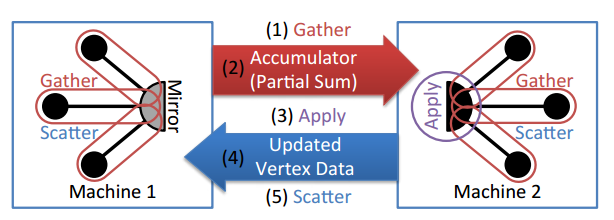
\includegraphics[width=\textwidth]{vertex_cut.png}\\
  \caption{The communication pattern of the PowerGraph abstraction when using a vertex-cut. Gather function runs locally on each machine and then one accumulators is sent from each
  mirror to the master. The master runs the apply function and
  then sends the updated vertex data to all mirrors. Finally the
  scatter phase is run in parallel on mirrors.}\label{vertex_cut}
\end{figure}



\section{Graphchi}
\subsection{Parallel Sliding Windows}

Parallel Sliding Windows (PSW)
method (Algorithm 2). PSW can process a graph with
mutable edge values efficiently from disk, with only a small
number of non-sequential disk accesses, while supporting
the asynchronous model of computation. PSW processes
graphs in three stages: it 1) loads a subgraph from disk; 2)
updates the vertices and edges; and 3) writes the updated
values to disk. These stages are explained in detail below,
with a concrete example. We then present an extension to
graphs that evolve over time, and analyze the I/O costs of
the PSW method

\begin{figure}
  \centering
  % Requires \usepackage{graphicx}
  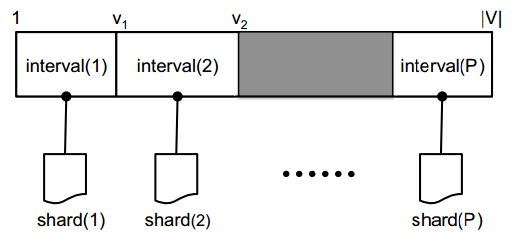
\includegraphics[width=\textwidth]{vertex_interval}\\
  \caption{The vertices of graph(V,E)are divided intoP
intervals. Each interval is associated with a shard, which
stores all edges that have destination vertex in that interval.}\label{vertex_int}
\end{figure}


Under the PSW method, the verticesV of graphG=
(V,E)are split intoPdisjointintervals. For each interval,
we associate ashard, which stores all the edges that have
destinationin the interval. Edges are stored in the order of
theirsource(Figure 1). Intervals are chosen to balance the
number of edges in each shard; the number of intervals,P,
is chosen so that any one shard can be loaded completely
into memory. Similar data layout for sparse graphs was
used previously, for example, to implement I/O efficient
Pagerank and SpMV [5, 21].
PSW does graph computation inexecution intervals,
by processing vertices one interval at a time. To create the
subgraph for the vertices in intervalp, their edges (with
their associated values) must be loaded from disk. First,
Shard(p), which contains the in-edges for the vertices
in interval(p), is loaded fully into memory. We call thus
shard(p) thememory-shard. Second, because the edges
are ordered by their source, theout-edgesfor the vertices
are stored in consecutive chunks in the other shards, requiring additionalP?1block reads. Importantly, edges for
interval(p+1) are stored immediately after the edges for
interval(p). Intuitively, when PSW moves from an interval
to the next, itslidesawindowover each of the shards. We
call the other shards thesliding shards. Note, that if the
degree distribution of a graph is not uniform, the window
length is variable. In total, PSW requires onlyPsequential
disk reads to process each interval. A high-level illustration
of the process is given in Figure 2, and the pseudo-code of
the subgraph loading is provided in Algorithm 3.

\begin{figure}
  \centering
  % Requires \usepackage{graphicx}
  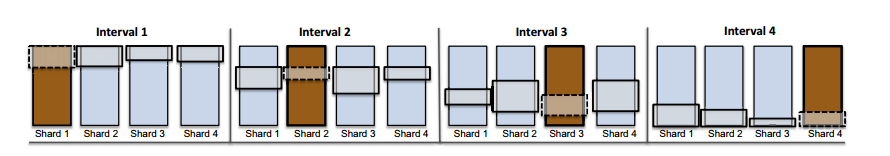
\includegraphics[width=\textwidth]{PSW.png}\\
  \caption{Visualization of the stages of one iteration of the Parallel Sliding Windows method. In this example, vertices
are divided into four intervals, each associated with a shard. The computation proceeds by constructing a subgraph of
vertices one interval a time. In-edges for the vertices are read from thememory-shard(in dark color) while out-edges
are read from each of thesliding shards. The currentsliding windowis pictured on top of each shard.}\label{PSW}
\end{figure}



After the subgraph for intervalphas been fully loaded from
disk, PSW executes the user-definedupdate-functionfor
each vertexin parallel. As update-functions can modify the
edge values, to prevent adjacent vertices from accessing
edges concurrently (race conditions), we enforceexternal
determinism, which guarantees that each execution of PSW
produces exactly the same result. This guarantee is straightforward to implement: vertices that have edges with both
end-points in the same interval are flagged ascritical, and
are updated in sequential order. Non-critical vertices do
not share edges with other vertices in the interval, and
can be updated safely in parallel. Note, that the update of
a critical vertex will observe changes in edges done by
preceding updates, adhering to theasynchronousmodel of
computation. This solution, of course, limits the amount of
effective parallelism. For some algorithms, consistency is
not critical (for example, see [29]), and we allow the user
to enable fully parallel updates.

Finally, the updated edge values need to be written to disk
and be visible to the next execution interval. PSW can do
this efficiently: The edges are loaded from disk in large
blocks, which are cached in memory. When the subgraph
for an interval is created, the edges are referenced as pointers to the cached blocks; modifications to the edge values
directly modify the data blocks themselves. After finishing the updates for the execution interval, PSW writes the
modified blocks back to disk, replacing the old data. The
memory-shard is completely rewritten, while only the activesliding windowof each sliding shard is rewritten to
disk (see Algorithm 2). When PSW moves to the next interval, it reads the new values from disk, thus implementing
the asynchronous model. The number of non-sequential
disk writes for a execution interval isP, exactly same as the
number of reads. Note, if an algorithm only updates edges
in one direction, PSW only writes the modified blocks to
disk.




\end{document}
